% ==============================================================================
% فصل چهارم: طراحی بستر سخت‌افزاری و ثبت سیگنال‌های فیزیکی \lr{Trace}
% ==============================================================================

\chapter{طراحی بستر سخت‌افزاری و ثبت سیگنال‌های فیزیکی \lr{Trace}}
\label{ch:hardware}

\section{مقدمه}
سیگنال‌های درگاه ردیابی موازی (\lr{Parallel Trace Port}) از حیث ماهیت الکتریکی، در رده سیگنال‌های دیجیتال فرکانس بالا قرار می‌گیرند. در این فرکانس‌ها، فرضیات ایده‌آل مدارهای متمرکز جای خود را به پدیده‌های خطوط انتقال، اعوجاج شکل‌موج، خازن‌ها و سلف‌های پارازیتی و تداخل متقابل سیگنال‌ها (\lr{Crosstalk}) می‌دهند. از سوی دیگر، شرایط تحریم و کمبود تجهیزات آزمایشگاهی پیشرفته در کشور، مانع بزرگی بر سر دستیابی به بردهای ارزیابی گران‌قیمت صنعتی به شمار می‌رفت. 

در این پژوهش، مسیر توسعه بستر سخت‌افزاری شامل دو فاز عملیاتی بود: در فاز نخست، به دلیل نبود گزینه‌های تجاری مناسب، یک هدربرد دست‌ساز با سیم‌کشی دستی بر روی برد هزارسوراخ توسعه داده شد که با چالش‌های متعدد نویز، ناپایداری در پروگرم کردن و شکنندگی اتصالات فیزیکی روبرو بود. در فاز دوم و با گذر زمان، یک هدربرد استاندارد تجاری از میکروکنترلر \lr{STM32H750VBT6} در بازار داخلی در دسترس قرار گرفت و با جایگزینی آن، تمامی موانع فیزیکی و سیگنالی برطرف گردید. 

در این فصل، چالش‌های ساخت هدربرد دست‌ساز، مشخصات فنی و مداری هدربرد تجاری، تمهیدات یکپارچگی سیگنال (\lr{Signal Integrity})، معماری سمپلینگ ۱۰ برابری با لاجیک‌آنالایزر \lr{DSLogic U3Pro16}، مشاهدات تجربی تغییر دیوتی‌سایکل و توجیه تئوری آن بر پایه خطای کوانتیزاسیون دیجیتال، و در نهایت دلایل بنیادین رد استفاده از درگاه تک‌سیمه \lr{Serial Wire} جهت دریافت \lr{Trace} تشریح می‌گردد.

\section{چالش دسترسی سخت‌افزاری و ساخت هدربرد دست‌ساز اولیه}
\label{sec:hw_board_challenge}
در آغاز پروژه، بررسی گزینه‌های سخت‌افزاری موجود برای میکروکنترلرهای سری \lr{Cortex-M7} شرکت \lr{STMicroelectronics} نتایج مأیوس‌کننده‌ای به همراه داشت:
\begin{enumerate}
    \item \textbf{بردهای ارزیابی رسمی (\lr{STM32H743I-EVAL} و \lr{Keil MCBSTM32H7}):} این بردها مجهز به کانکتورهای اختصاصی ۲۰ پین و ۳۸ پین ردیابی (\lr{MICTOR / CoreSight 20}) هستند؛ اما قیمت آن‌ها بیش از ۵۰۰ تا ۱۰۰۰ دلار بوده و به دلیل محدودیت‌های وارداتی و تحریمی، امکان تهیه آن‌ها برای یک پروژه دانشگاهی در بازه زمانی معقول وجود نداشت.
    \item \textbf{بردهای عمومی دیسکاوری و نوکلئو (\lr{NUCLEO-144}):} اگرچه بردهایی نظیر \lr{NUCLEO-H743ZI} در بازار یافت می‌شدند، اما پایه‌های درگاه \lr{TPIU} (به‌ویژه پایه‌های پورت \lr{E} یعنی \texttt{PE2} الی \texttt{PE6}) بر روی این بردها به صورت مشترک با مدارهای کنترلر فیزیکی اترنت (\lr{Ethernet PHY})، کریستال‌های فرعی یا سوکت‌های هدر \lr{Arduino} متصل شده بودند. اتصال این پایه‌ها از مسیرهای طولانی، بدون محافظ و با خازن پارازیتی بالا بر روی برد، شکل‌موج کلاک ردیابی را کاملاً دفرمه می‌کرد و مانع ثبت پایدار داده‌ها می‌شد.
\end{enumerate}

با توجه به این بن‌بست، در فاز نخست پروژه تصمیم گرفته شد یک هدربرد اولیه به صورت کاملاً دست‌ساز بر روی برد هزارسوراخ (\lr{Perfboard}) با استفاده از یک برد مبدل تبدیل پکیج \lr{LQFP100} به پایه‌های دیپ (\lr{DIP}) ساخته و سیم‌کشی گردد. در این مدار، پایه‌های تغذیه، خازن‌های دی‌کوپلینگ، کریستال خارجی، مدار ریست و اتصالات پین‌هدرها با سیم‌بندی دستی نقطه‌به‌نقطه اجرا شد. همچنین یک ماژول تغذیه کاهنده دی‌سی به دی‌سی (\lr{Buck Converter}) با پورت ورودی \lr{USB} برای تأمین ولتاژ پایدار ۳.۳ ولت بر روی برد تعبیه گردید.

اگرچه این هدربرد دست‌ساز امکان راه‌اندازی اولیه و اجرای نخستین آزمایش‌های کلاک را فراهم ساخت، اما در عمل با چالش‌های فنی شدیدی مواجه شد:
\begin{itemize}
    \item \textbf{نویز شدید بر روی خطوط \lr{Trace}:} به دلیل فقدان صفحه زمین (\lr{Ground Plane}) یکپارچه و وجود سلف‌ها و خازن‌های پارازیتی ناشی از سیم‌های معلق، شکل‌موج کلاک \lr{Trace} دچار جهش‌های ولتاژی، نوسانات میرای فرکانس بالا (\lr{Ringing}) و جهش زمین (\lr{Ground Bounce}) می‌شد که منجر به خطا در ثبت بسته‌ها می‌گردید.
    \item \textbf{مشکلات و بی‌ثباتی در پروگرم کردن میکروکنترلر:} رابط برنامه‌ریزی \lr{SWD} با نویزهای القایی محیطی تداخل پیدا می‌کرد و پروگرامر \lr{ST-Link} مکرراً ارتباط خود را با پردازنده از دست می‌داد یا در شناسایی شناسه تراشه با شکست مواجه می‌شد.
    \item \textbf{سختی اتصالات فیزیکی و شکنندگی مکانیکی:} سیم‌کشی‌های متعدد بر روی برد هزارسوراخ در اثر کوچک‌ترین جابجایی یا اتصال پروب‌های تست دچار قطعی، شکستگی یا اتصالی ناخواسته می‌شدند و زمان زیادی صرف عیب‌یابی مداوم اتصالات می‌گردید.
\end{itemize}

ساختار کلی بلوک‌های سخت‌افزاری مورد نیاز و ارتباطات بخش‌های مختلف هدربرد در شکل \ref{fig:custom_board_block} نشان داده شده است. همچنین تصویر هدربرد دست‌ساز اولیه پیاده‌سازی‌شده بر روی برد هزارسوراخ در شکل \ref{fig:board_handmade} به تصویر کشیده شده است.

\begin{figure}[H]
\centering
\begin{latin}
\begin{tikzpicture}[
    box/.style={rectangle, draw=black!70, fill=gray!8, thick, rounded corners=4pt, text width=5.8cm, align=right, inner sep=5pt},
    header/.style={rectangle, draw=blue!80, fill=blue!10, thick, rounded corners=4pt, text width=5.8cm, align=right, inner sep=5pt},
    pwr/.style={rectangle, draw=red!70, fill=red!8, thick, rounded corners=4pt, text width=5.8cm, align=right, inner sep=5pt}
]
    \node [box] (mcu) {\textbf{\rl{هسته پردازشی مرکزی}}\\\lr{STM32H750VBT6 (LQFP100)}\\\small \rl{کلاک سیستم تا ۴۸۰ مگاهرتز،} \lr{128KB} \rl{فلش،} \lr{1MB} \rl{رم}};
    
    \node [header, right=0.8cm of mcu] (trace) {\textbf{\rl{خطوط درگاه \lr{Trace} (۵ سیم)}}\\\lr{TRACECLK (PE2), TRACED0..3 (PE3..6)}\\\small \rl{اتصال مستقیم به همراه پین‌های زمین مجاور}};
    
    \node [pwr, below=0.8cm of mcu] (power) {\textbf{\rl{زیرسیستم تغذیه و دی‌کوپلینگ}}\\\small \rl{خازن‌های چندلایه سرامیکی} \lr{100nF}\\\small \rl{رگولاتور خطی ۳.۳ ولت و مسیرهای زمین پیوسته}};
    
    \node [box, below=0.8cm of trace] (clock) {\textbf{\rl{اسیلاتور و کلاک مرجع}}\\\small \rl{کریستال خارجی} \lr{25MHz HSE}\\\small \rl{خازن‌های بار ۱۸ پیکوفاراد}};

    \draw [-latex, very thick] (mcu) -- (trace);
    \draw [-latex, very thick] (power) -- (mcu);
    \draw [-latex, very thick] (clock) -- (mcu);
\end{tikzpicture}
\end{latin}
\caption{بلوک دیاگرام معماری سخت‌افزار هدربرد و اتصالات درگاه \lr{Trace}}
\label{fig:custom_board_block}
\end{figure}

\begin{figure}[H]
\centering
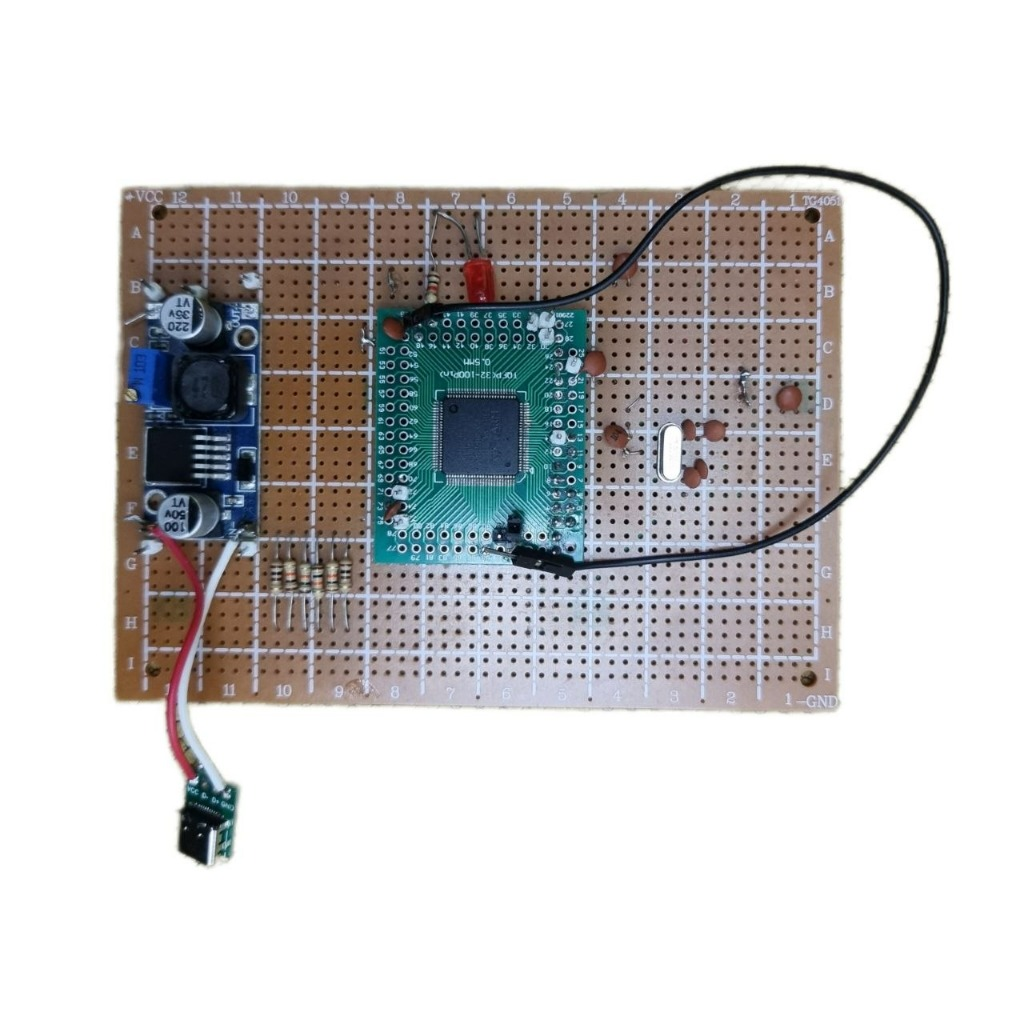
\includegraphics[height=5.2cm, keepaspectratio]{figures/board_handmade_perfboard.jpg}
\caption{هدربرد دست‌ساز اولیه پیاده‌سازی‌شده بر روی برد هزارسوراخ}
\label{fig:board_handmade}
\end{figure}

\section{گذار به هدربرد تجاری \lr{STM32H750VBT6} و مشخصات فنی آن}
\label{sec:commercial_board_transition}
با گذر زمان و پیگیری‌های مستمر، یک هدربرد ساده و استاندارد تجاری از میکروکنترلر \lr{STM32H750VBT6} در بازار داخلی موجود شد و بلافاصله خریداری گردید. از آن پس، تمامی فرآیندهای توسعه نرم‌افزاری و سخت‌افزاری بر روی این هدربرد هدایت شد.

ورود هدربرد تجاری، جهش بزرگی در کیفیت و پایداری آزمایش‌ها ایجاد کرد؛ به‌طوری‌که چالش‌های پروگرم کردن تراشه، نویز خطوط \lr{Trace}، سختی اتصالات و شکنندگی مکانیکی کاملاً برطرف شده و دیگر چالشی در مسیر پروژه محسوب نمی‌شدند. شکل \ref{fig:board_commercial} هدربرد تجاری تهیه‌شده را نشان می‌دهد که دارای پکیج ۱۰۰ پایه \lr{LQFP} و جانمایی استاندارد است.

\begin{figure}[H]
\centering
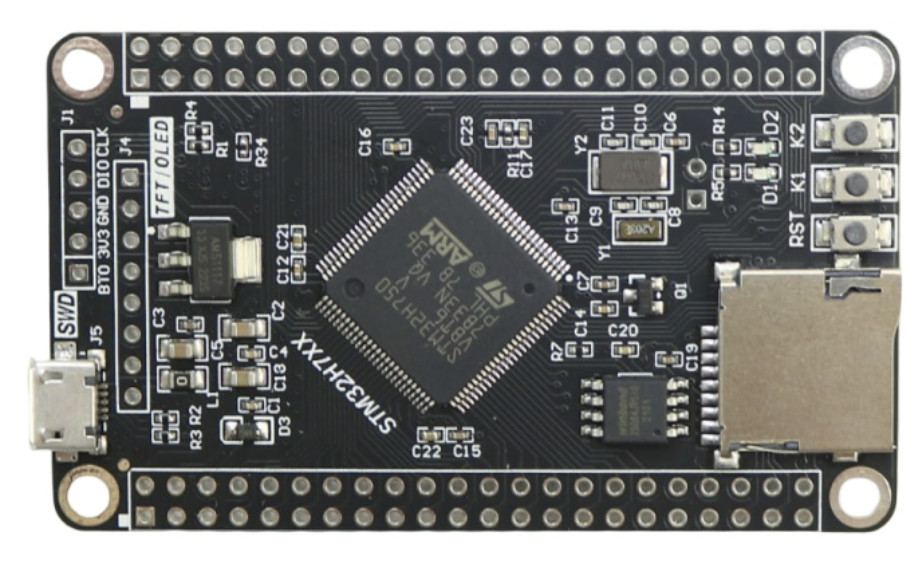
\includegraphics[height=5.5cm, keepaspectratio]{figures/board_commercial_h750.png}
\caption{هدربرد استاندارد تجاری \lr{STM32H750VBT6}}
\label{fig:board_commercial}
\end{figure}

\subsection{تخصیص پایه‌ها و مسیرکشی اختصاصی \lr{Trace}}
پایه‌های ردیابی موازی ۴ بیتی در تراشه \lr{STM32H750} بر روی پورت \lr{E} قرار دارند. جدول \ref{tab:tpiu_pins} مشخصات سیگنال‌ها و جانمایی پایه‌ها را به همراه خط‌کشی کامل نمایش می‌دهد:

\begin{table}[ht]
\centering
\caption{تخصیص پایه‌های فیزیکی میکروکنترلر \lr{STM32H750VBT6} به درگاه \lr{TPIU}}
\label{tab:tpiu_pins}
\begin{tabularx}{\textwidth}{|l|c|c|c|X|}
\hline
\textbf{پایه تراشه} & \textbf{شماره پین} & \textbf{سیگنال \lr{TPIU}} & \textbf{تابع جایگزین} & \textbf{پیکربندی درگاه} \\
\hline
\texttt{PE2} & پین ۱ & \texttt{TRACECLK} & \lr{AF0} & \lr{Very High Speed (100MHz+)} \\
\hline
\texttt{PE3} & پین ۲ & \texttt{TRACED0} & \lr{AF0} & \lr{Very High Speed (100MHz+)} \\
\hline
\texttt{PE4} & پین ۳ & \texttt{TRACED1} & \lr{AF0} & \lr{Very High Speed (100MHz+)} \\
\hline
\texttt{PE5} & پین ۴ & \texttt{TRACED2} & \lr{AF0} & \lr{Very High Speed (100MHz+)} \\
\hline
\texttt{PE6} & پین ۵ & \texttt{TRACED3} & \lr{AF0} & \lr{Very High Speed (100MHz+)} \\
\hline
\end{tabularx}
\end{table}

یکی از مزایای مهم فیزیکی پکیج \lr{LQFP100} در این تراشه، مجاورت پایه‌های ۱ تا ۵ با یکدیگر در گوشه سمت چپ بالای آی‌سی است. این امر باعث می‌شود که خطوط کلاک و داده ردیابی در کمترین فاصله ممکن به پین‌هدرهای لبه برد برسند و تطبیق طول مسیرها با کمترین اختلاف فاز ممکن میسر گردد.

\subsection{ملاحظات دی‌کوپلینگ و پایداری تغذیه}
تغییر وضعیت همزمان ۵ پین دیجیتال در فرکانس بالا با نرخ تغییر ولتاژ حداکثری، جریانی لحظه‌ای به ریل‌های تغذیه وارد می‌کند. در هدربرد تجاری خریداری‌شده، وجود صفحه زمین پیوسته و خازن‌های سرامیکی \lr{100nF} چندلایه (\lr{MLCC}) در نزدیکی پایه‌های \texttt{VDD/VSS}، پدیده جهش زمین را به حداقل رسانده و مسیر برگشت جریان را با کمترین اندوکتانس حلقه مسدود ساخته است.

\section{یکپارچگی سیگنال در کابل‌های رابط و پروب‌ها}
برای انتقال سیگنال‌ها از هدربرد به ابزار دریافت لاجیک، اصول یکپارچگی سیگنال مد نظر قرار گرفت:
\begin{enumerate}
    \item \textbf{طول کابل‌های اتصال:} استفاده از کابل‌های بلند رابط به دلیل ایجاد اندوکتانس پارازیتی موجب نوسانات پله‌ای (\lr{Ringing}) و خوانش اشتباه سطوح منطقی می‌گردد. بنابراین، طول کابل‌های پروب به کمتر از ۱۰ سانتی‌متر محدود گردید.
    \item \textbf{تنظیم ثبّات نرخ خیز خروجی (\lr{OSPEEDR}):} ثبّات \lr{GPIOE\_OSPEEDR} برای تمام پایه‌های \texttt{PE2..PE6} بر روی وضعیت «سرعت بسیار بالا» (\lr{0b11 - Very High Speed}) تنظیم شد تا زمان خیز و افت پالس‌ها به حداقل رسیده و لبه‌های کلاک به صورت کاملاً شارپ شکل گیرند.
\end{enumerate}

\section{معماری سمپلینگ با فرکانس متناسب (سمپلینگ ۱۰ برابری)}
\label{sec:sampling_strategy}
در سامانه‌های صنعتی مجهز به پروب‌های سخت‌افزاری پیشرفته، دیباگر مستقیماً با کلاک سنکرون تراشه در فرکانس‌های ۱۰۰ مگاهرتز به بالا هماهنگ می‌شود. اما در سناریوی استفاده از لاجیک‌آنالایزرهای عمومی اقتصادی، این رویکرد به دلیل تغییرات فاز کلاک و عدم تطبیق زمان برپایی و نگه‌داری (\lr{Setup \& Hold Time}) منجر به پرش بیت‌ها می‌گردد. برای دستیابی به اطمینان ۱۰۰ درصدی، استراتژی سمپلینگ ناهمگام با نرخ متناسب ۱۰ برابری اتخاذ گردید.

\subsection{مشخصات لاجیک‌آنالایزر \lr{DSLogic U3Pro16}}
\label{sec:dslogic_hw}
برای ثبت سیگنال‌های درگاه ردیابی، از لاجیک‌آنالایزر پرسرعت \lr{DSLogic U3Pro16} ساخت شرکت \lr{DreamSourceLab} استفاده شد. این دستگاه دارای ۱۶ کانال ورودی دیجیتال، ارتباط پرسرعت \lr{USB 3.0} و حافظه داخلی \lr{2Gb DDR3 DRAM} است که امکان نمونه‌برداری با فرکانس‌های بالا را بدون افت فریم در بافر داخلی فراهم می‌کند. شکل \ref{fig:dslogic_hardware} این دستگاه را نمایش می‌دهد.

\begin{figure}[ht]
\centering
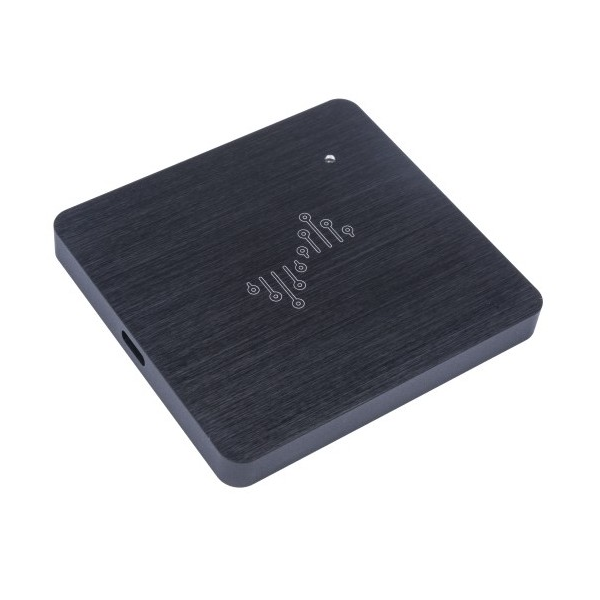
\includegraphics[width=0.62\textwidth]{figures/dslogic_u3pro16.png}
\caption{لاجیک‌آنالایزر سخت‌افزاری \lr{DSLogic U3Pro16} با رابط پرسرعت \lr{USB 3.0} و حافظه داخلی \lr{DRAM}}
\label{fig:dslogic_hardware}
\end{figure}

\subsection{استراتژی سمپلینگ ۱۰ برابری و استخراج پایدار داده‌ها}
\label{sec:sampling_technique}
برای تضمین دریافت بیست‌درصدی داده‌ها و حذف کامل خطای فاز:
\begin{itemize}
    \item کلاک پردازنده و کلاک خروجی درگاه ردیابی در یک پله کاری پایدار (مانند ۱۰ مگاهرتز یا کلاک مقیاس‌شده ۱ مگاهرتز) تنظیم می‌گردد.
    \item لاجیک‌آنالایزر با نرخ نمونه‌برداری \textbf{۱۰ برابری} (به عنوان مثال ۱۰۰ مگاهرتز برای کلاک ردیابی ۱۰ مگاهرتز) خطوط \texttt{TRACECLK} و \texttt{TRACED[0:3]} را اسکن می‌نماید.
\end{itemize}

همان‌طور که در شکل \ref{fig:sampling_concept} مشاهده می‌شود، سمپلینگ با ضریب ۱۰ برابری مزایای بنیادینی به همراه دارد:
\begin{enumerate}
    \item هر نیم‌پریود کلاک شامل حداقل ۵ نمونه دیجیتال است؛ بنابراین نرم‌افزار میزبان لبه‌های بالارونده و پایین‌رونده را بدون تأثیرپذیری از نویزهای ضربه‌ای تک‌نمونه‌ای شناسایی می‌کند.
    \item خطوط داده (\lr{TRACED[0:3]}) در نمونه میانی (نمونه سوم در پنجره ۵ نمونه‌ای) خوانده می‌شوند؛ یعنی دقیقاً در مرکز چشم‌پالس الکتریکی (\lr{Eye Diagram}) که سیگنال به بیشترین ثبات ولتاژی رسیده و زمان‌های برپایی و نگه‌داری کاملاً ارضا شده‌اند.
\end{enumerate}

\begin{figure}[ht]
\centering
\begin{latin}
\begin{tikzpicture}[xscale=0.78, yscale=0.9]
    % Clock wave
    \draw[thick, black] (0,2) -- (2,2) -- (2,0) -- (4,0) -- (4,2) -- (6,2) -- (6,0) -- (8,0) -- (8,2) -- (10,2);
    \node[left] at (0,1) {\texttt{TRACECLK}};
    
    % Data wave
    \draw[thick, blue] (0,0.5) -- (1.8,0.5) -- (2.2,1.5) -- (5.8,1.5) -- (6.2,0.5) -- (10,0.5);
    \node[left] at (0,-0.5) {\texttt{TRACED[0:3]}};
    \node[blue] at (4,1.0) {\small \rl{نیبل معتبر} (Nibble Data)};
    
    % Sampling ticks (10x sampling)
    \foreach \x in {0.2, 0.6, 1.0, 1.4, 1.8, 2.2, 2.6, 3.0, 3.4, 3.8, 4.2, 4.6, 5.0, 5.4, 5.8, 6.2, 6.6, 7.0, 7.4, 7.8, 8.2, 8.6, 9.0, 9.4, 9.8} {
        \draw[red!70, dashed] (\x, -1.0) -- (\x, 2.3);
        \fill[red] (\x, -1.0) circle (1.5pt);
    }
    \node[right, red!80!black] at (10,-1.0) {\small \rl{نمونه‌های ۱۰ برابری} (10x Samples)};
    
    % Optimal sampling point
    \draw[latex-, very thick, green!50!black] (3.0,1.55) -- (3.0,2.6) node[above, font=\small, text=green!50!black] {\rl{نقطه پایدار نمونه‌برداری در مرکز چشم}};
\end{tikzpicture}
\end{latin}
\caption{نمودار زمانی تکنیک سمپلینگ ۱۰ برابری و استخراج پایدار داده‌ها در مرکز چشم الکتریکی}
\label{fig:sampling_concept}
\end{figure}

\subsection[مشاهدات تجربی دیوتی‌سایکل و کوانتیزاسیون]{مشاهدات تجربی دیوتی‌سایکل و توجیه تئوری کوانتیزاسیون دیجیتال}
\label{sec:duty_cycle_quantization}
در مراحل اولیه آزمایش‌های عملی، پدیده‌ای جالب توجه در ثبت سیگنال کلاک \lr{Trace} مشاهده شد: هنگامی که یک سیگنال کلاک با فرکانس اسمی ۱۰ مگاهرتز (پریود ۱۰۰ نانوثانیه) با نرخ نمونه‌برداری ۱۰۰ مگاهرتز (۱۰ برابر فرکانس سیگنال) ثبت می‌شد، مقادیر دیوتی‌سایکل اندازه‌گیری‌شده توسط نرم‌افزار لاجیک‌آنالایزر همواره ثابت نبود. در برخی دوره‌ها، دیوتی‌سایکل دقیقاً ۵۰ درصد (\lr{50.00\%}) با عرض پالس مثبت ۵۰ نانوثانیه بود (شکل \ref{fig:dslogic_duty50})؛ اما در سایر دوره‌ها یا نمونه‌برداری‌های دیگر، این مقدار به اعدادی نظیر ۴۰ درصد (\lr{40.00\%} در شکل \ref{fig:dslogic_duty40})، ۶۰ درصد، ۵۶ درصد یا مقادیر نامتقارن دیگر تغییر می‌کرد.

\begin{figure}[ht]
\centering
\begin{subfigure}[b]{0.48\textwidth}
    \centering
    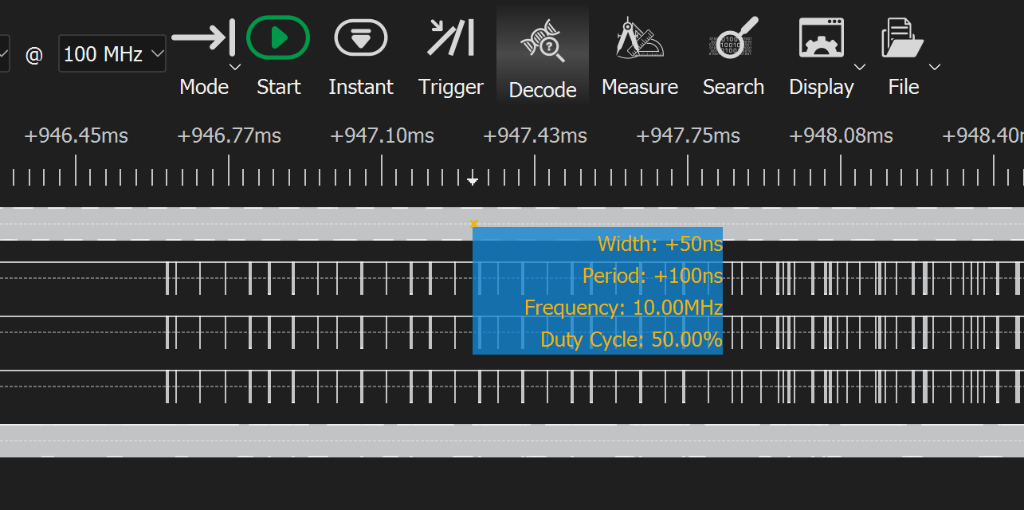
\includegraphics[width=\textwidth]{figures/dslogic_duty50.png}
    \caption{نمونه‌برداری با دیوتی‌سایکل متقارن ۵۰ درصد (\lr{Width: +50ns})}
    \label{fig:dslogic_duty50}
\end{subfigure}
\hfill
\begin{subfigure}[b]{0.48\textwidth}
    \centering
    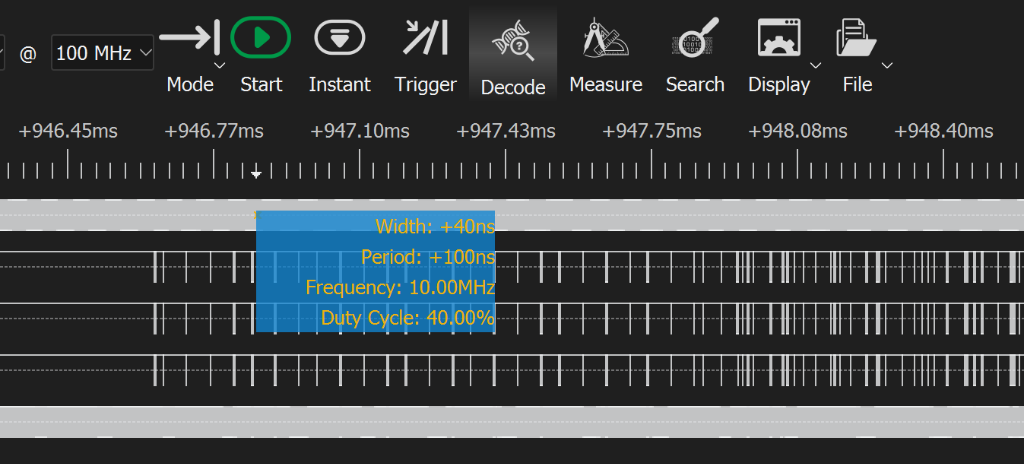
\includegraphics[width=\textwidth]{figures/dslogic_duty40.png}
    \caption{نمونه‌برداری با دیوتی‌سایکل نامتقارن ۴۰ درصد (\lr{Width: +40ns})}
    \label{fig:dslogic_duty40}
\end{subfigure}
\caption{مشاهدات تجربی اندازه‌گیری کلاک \lr{Trace} ۱۰ مگاهرتز توسط لاجیک‌آنالایزر در نرخ نمونه‌برداری ۱۰۰ مگاهرتز}
\label{fig:dslogic_duty_comparison}
\end{figure}

با بررسی دقیق فرآیند نمونه‌برداری لاجیک‌آنالایزر و مراجعه به راهنمای کاربری سازنده (\lr{DreamSourceLab DSView User Guide}) \cite{dslab2023dsview}، مشخص گردید که این نوسان دیوتی‌سایکل ناشی از \textbf{طبیعت دیجیتال و ناهمگام نمونه‌برداری گسسته در زمان} (\lr{Asynchronous Discrete-Time Quantization}) است و نشان‌دهنده تغییر فیزیکی در سیگنال خروجی میکروکنترلر نیست. دلایل تئوری این رخداد به شرح زیر تبیین می‌گردد:
\begin{enumerate}
    \item \textbf{خطای کوانتیزاسیون زمانی (\lr{Timing Quantization Uncertainty}):} لاجیک‌آنالایزر مجهز به اسیلاتور محلی خود است که مستقل از کلاک میکروکنترلر عمل می‌کند. در نرخ نمونه‌برداری ۱۰۰ مگاهرتز، فاصله زمانی بین دو نمونه متوالی $T_s = 10\,\mathrm{ns}$ است. از آنجا که لبه واقعی پالس کلاک می‌تواند در هر نقطه‌ای میان دو تیک نمونه‌برداری رخ دهد، بر اساس اصل نمونه‌برداری دیجیتال، عدم قطعیت در تشخیص هر لبه معادل $\pm T_s$ یعنی $\pm 10\,\mathrm{ns}$ خواهد بود \cite{dslab2023dsview}.
    \item \textbf{توزیع نمونه‌ها در یک دوره پریودیک:} در یک دوره تناوب ۱۰۰ نانوثانیه‌ای، دقیقاً ۱۰ نمونه ثبت می‌شود. اگر فاز کلاک نمونه‌برداری به‌طور متقارن با سیگنال ورودی قفل شده باشد، ۵ نمونه در سطح بالا (\lr{High}) و ۵ نمونه در سطح پایین (\lr{Low}) قرار می‌گیرند که دیوتی‌سایکل را ۵۰ درصد نشان می‌دهد ($5 \times 10\,\mathrm{ns} = 50\,\mathrm{ns}$). اما یک جابجایی زمانی ناچیز، لغزش فاز یا جیتر به میزان چند نانوثانیه کافی است تا یکی از نمونه‌های نزدیک به لبه تغییر وضعیت داده و تعداد نمونه‌های سطح بالا به ۴ و سطح پایین به ۶ برسد؛ در نتیجه دیوتی‌سایکل اندازه‌گیری‌شده برابر ۴۰ درصد ($4 \times 10\,\mathrm{ns} = 40\,\mathrm{ns}$) گزارش می‌شود.
    \item \textbf{توجیه نیاز به سمپلینگ ۱۰ برابری بر پایه مستندات سازنده:} در راهنمای رسمی لاجیک‌آنالایزر \cite[بخش ۲.۳.۲ و شکل ۲-۱۰]{dslab2023dsview} صراحتاً بیان شده است که با ضریب نمونه‌برداری کمتر (نظیر ۲ یا ۵ برابر)، خطای زمانی به $1/2 T$ یا $1/5 T$ می‌رسد که می‌تواند به از دست رفتن کامل پالس‌ها (\lr{Pulse Loss}) یا اعوجاج شدید دیوتی‌سایکل (نظیر نسبت‌های ۳ به ۲ یا ۵ به ۳) منجر شود. در مقابل، سمپلینگ با ضریب ۱۰ برابری خطای فاز را به کمتر از ۱۰ درصد ($\pm 10\%$) محدود کرده و تضمین می‌نماید که تمامی لبه‌ها بدون پرش بیت شناسایی شوند. این تطابق کامل مشاهدات تجربی با روابط تئوری کوانتیزاسیون، مهر تأییدی بر کفایت و ضرورت ضریب ۱۰ برابری در این سامانه بود.
\end{enumerate}

\section{بررسی و دلایل رد درگاه \lr{Serial Wire} جهت دریافت \lr{Trace}}
\label{sec:rejection_of_swo}
در مراحل طراحی معماری سخت‌افزاری سامانه، این پرسش مطرح شد که آیا می‌توان به جای درگاه موازی چندسیمه \lr{TPIU}، داده‌های ردیابی را بر روی درگاه سریال \lr{Serial Wire (SW / SWO)} دریافت نمود تا از چالش‌های سیم‌کشی متعدد، ملاحظات فرکانس بالا و نیاز به لاجیک‌آنالایزر چندکاناله رهایی یافت؟ با ارزیابی دقیق معماری پردازنده و الزامات آزمون، این گزینه به دلایل قاطع زیر رد گردید:
\begin{enumerate}
    \item \textbf{پهنای باند بسیار بالای داده‌های \lr{Trace} دستورات (\lr{High Bandwidth of ETM Trace}):} ماژول ردیابی دستورات (\lr{ETMv4}) به ازای هر انشعاب برنامه، استثنا یا تغییر مسیر کنترلی، بسته‌های ردیابی اتم (\lr{Atom Packets}) و نشانی هدف تولید می‌کند. در پردازنده‌های مدرن فرکانس بالا، حجم این داده‌ها به ده‌ها مگابایت بر ثانیه می‌رسد. خط تک‌سیمه \lr{SWO} که در مدهای آسنکرون \lr{UART} یا منچستر کار می‌کند، دارای پهنای باند بسیار محدودی (معمولاً در محدوده چند مگابیت بر ثانیه) است و به سرعت دچار سرریز بافر و افت بسته‌ها (\lr{Packet Loss}) می‌گردد.
    \item \textbf{عدم وجود یا محدودیت بافر اختصاصی \lr{Trace} در تراشه (\lr{Lack of Trace Buffer}):} بسیاری از میکروکنترلرهای سری استاندارد (از جمله \lr{STM32H750}) فاقد بافرهای حجیم آن‌چیپ نظیر \lr{Embedded Trace Buffer (ETB)} یا \lr{Embedded Trace FIFO (ETF)} هستند تا بتوانند جریان کامل \lr{Trace} را در حافظه درونی متوقف و سپس به صورت قطره‌چکانی تخلیه کنند. بنابراین، داده‌های \lr{Trace} باید به صورت کاملاً بی‌درنگ و با کمترین تأخیر به دنیای خارج هدایت شوند که تنها از عهده درگاه موازی پرسرعت برمی‌آید.
    \item \textbf{اشغال انحصاری درگاه \lr{SW} توسط پروژه مکمل برای تبادل ورودی/خروجی:} حیاتی‌ترین دلیل رد این گزینه، وابستگی معماری کلان سامانه آزمون به درگاه \lr{SWD} بود. در این ساختار مشترک، پورت \lr{SW} (شامل پایه‌های \texttt{SWDIO} و \texttt{SWCLK}) به‌طور مداوم توسط پروژه مکمل جهت تزریق تحریک‌های تست (\lr{Test Stimuli}) به داخل ثبّات‌ها و خواندن مقادیر ورودی/خروجی و پاسخ‌های سخت‌افزار تحت آزمون استفاده می‌شد. اشغال این درگاه برای داده‌های حجیم ردیابی، به مسدود شدن کانال آزمون و بن‌بست ارتباطی منجر می‌گردید.
    \item \textbf{فقدان کلاک فیزیکی سنکرون و ناسازگاری با استاندارد \lr{Trace} دستورات:} پایه \lr{SWO} فاقد کلاک سنکرون فیزیکی (\texttt{TRACECLK}) است و در سطح سخت‌افزار تنها برای ارسال بسته‌های رویدادی ماژول‌های سبک‌تر نظیر \lr{ITM} (\lr{Instrumentation Trace}) و \lr{DWT} طراحی شده است؛ در حالی که ردیابی چرخه‌دقیق دستورات نیازمند گذرگاه همگام چندبیتی \lr{TPIU} با تضمین هم‌زمانی کلاک و داده است.
\end{enumerate}

بنابراین، پیاده‌سازی سخت‌افزاری مبتنی بر درگاه ۴ بیتی موازی \lr{TPIU} به همراه کلاک اختصاصی، تنها رویکرد ممکن و استاندارد برای دستیابی به ردیابی کامل و بی‌درنگ دستورات بدون تداخل با فرآیند آزمون نرم‌افزار ارزیابی گردید.

\section{جمع‌بندی فصل}
در این فصل، مسیر تکامل بستر سخت‌افزاری سامانه از هدربرد دست‌ساز اولیه ساخته‌شده بر روی برد هزارسوراخ تا گذار موفق به هدربرد استاندارد تجاری \lr{STM32H750VBT6} تبیین گردید. تمهیدات یکپارچگی سیگنال شامل کوتاه نگاه داشتن طول پروب‌ها و تنظیم خروجی‌های سرعت بسیار بالا شرح داده شد. سپس معماری سمپلینگ ۱۰ برابری با استفاده از لاجیک‌آنالایزر \lr{DSLogic U3Pro16} معرفی شد و پدیده تجربی تغییر دیوتی‌سایکل بر پایه تئوری کوانتیزاسیون دیجیتال ناهمگام و استانداردهای سازنده لاجیک‌آنالایزر توجیه گردید. در نهایت، دلایل فنی و عملیاتی رد درگاه \lr{Serial Wire} به نفع درگاه موازی \lr{TPIU} بررسی شد. در فصل پنجم، پیکربندی سطح پایین ثبّات‌های درونی میکروکنترلر و \lr{Firmware} مورد نیاز جهت فعال‌سازی این بستر سخت‌افزاری تشریح خواهد شد.
